\documentclass{exam}
\usepackage{amsmath}
\usepackage{amssymb}
\usepackage{amsthm}
\usepackage{graphicx}
\usepackage{float}
\usepackage{mathtools}


\begin{document}
\centering
\makebox[\textwidth]{\textsc{Fundamental Groups and Covering Spaces Midterm}}
\makebox[\textwidth]{\textsc{Fall 2021}}
\makebox[\textwidth]{\textsc{Keiko Kawamuro}}
\vspace{1em}
\begin{questions}
    \question
        Let $X=\mathbb{R}^3\setminus Z$ where $Z\subset\mathbb{R}^3$ is the $z$-axis (so $Z$ is homeomorphic to $\mathbb{R}$.) 
        Show that $X$ is not simply connected.
    \question
        Identify a torus $S^1 \times S^1$ with a square $S$ whose vertical sides are glued and horizontal sides are glued.
        \begin{parts}
            \part
               Sketch a loop (in the square $S$) that represents the element $(2,3) \in \mathbb{Z}\times\mathbb{Z} \cong\pi_1(S^1\times S^1)$.
            \part
                Do the same for $(6,4)$.
        \end{parts}
    \question
        Find a map $f: S^1 \to S^1$ that yields the mapping cylinder structure of a Möbius band.
    \question
        Let $f: I\to\mathbb{R}^3$ be a loop whose image is the unit circle and $g: I \to \mathbb{R}^3$ be a trefoil knot. Are $f$ and $g$ homotopic?
    \question
        Show that there are no retractions $r: X \to A$ in the following cases:
        \begin{parts}
            \part
                $X=S^1\times D^2$ and $A$ is the circle shown below.
                \begin{figure}[h!]
                    \centering
                    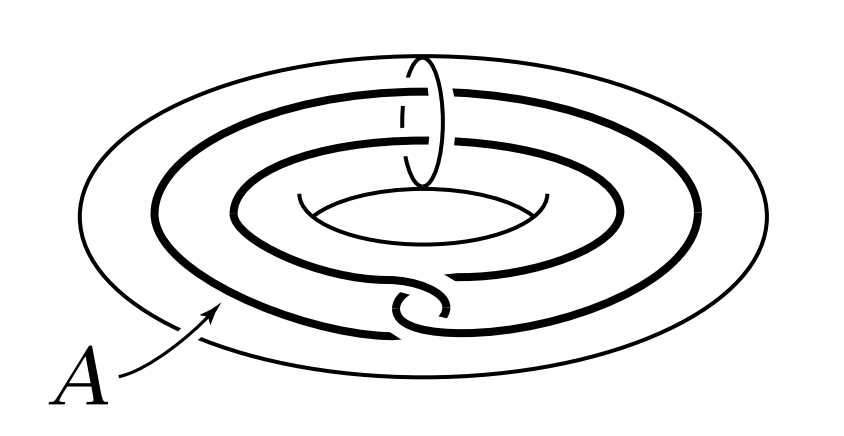
\includegraphics[width=0.5\textwidth]{torus_loop.png}
                  \end{figure}
            \part
                $X$ is the Möbius band and $A$ is the boundary of $X$.
        \end{parts}
    \question
        \begin{parts}
            \part
                Find a cell-complex structure of a genus 2 orientable surface.
            \part
                Do the same for general genus $g$.
        \end{parts}
\end{questions}
\end{document}